\documentclass[conference]{IEEEtran}
\IEEEoverridecommandlockouts

\usepackage{cite}
\usepackage{amsmath,amssymb,amsfonts}
\usepackage{algorithmic}
\usepackage{graphicx}
\usepackage{textcomp}
\usepackage{xcolor}
\usepackage{booktabs}
\usepackage{multirow}
\usepackage{url}
\usepackage[hidelinks]{hyperref}

\def\BibTeX{{\rm B\kern-.05em{\sc i\kern-.025em b}\kern-.08em
    T\kern-.1667em\lower.7ex\hbox{E}\kern-.125emX}}

\begin{document}

\title{FaithfulX-Derm: Stability and Faithfulness of Grad-CAM and
Integrated Gradients Explanations for Skin Lesion Classification\\
{\footnotesize An empirical study with null-calibrated perturbations and
held-out test validation}
}

\author{
\IEEEauthorblockN{Gaurang Gupta; Gaurav Kohli}
\IEEEauthorblockA{\textit{Department of Computer Science and Engineering, NSUT, New Delhi, India}}
}

\maketitle

\begin{abstract}
Post-hoc explanation methods such as Grad-CAM and Integrated Gradients (IG)
are increasingly applied to clinical image classifiers, but their stability
under input perturbations and their faithfulness to model behaviour are
incompletely characterised. We train a ResNet-18 on HAM10000 (7 classes,
10,015 images) and perturb 166 validation images with six perturbation types
at two severities, plus two near-identity null controls. We measure
explanation stability (Spearman correlation, cosine similarity, top-20\%
overlap), faithfulness (deletion and insertion gaps against a random-order
control), and whether explanation instability helps detect misclassified
images beyond model confidence. Noise is the most disruptive perturbation
for predictions (63.3\% flipped at severity 2), and a JPEG q=95 control
assumed harmless is not inert (16.3\% flipped on validation, 10.3\% on
test). Neither explanation method is clearly more stable: under severe
noise, Grad-CAM produced an all-zero map for 28.3\% of validation images,
only where the prediction had flipped. Scoring these as zero similarity, IG
appears more stable on Spearman correlation; excluding them, the methods are
statistically indistinguishable (0.769 vs 0.739). Both methods beat
random-order deletion and insertion with modest gaps. In this setting (one
model, one dataset, 60 validation errors) we found no evidence that
explanation instability adds information beyond confidence (AUROC 0.737 for
confidence, 0.616 for Grad-CAM instability, and 0.473 for IG, which is
indistinguishable from chance). Findings were directionally consistent on a
held-out test split (165 images).
\end{abstract}

\begin{IEEEkeywords}
explainable AI, Grad-CAM, integrated gradients, skin lesion classification,
HAM10000, explanation stability, faithfulness, deletion and insertion,
uncertainty, model error detection
\end{IEEEkeywords}

\section{Introduction}

Automated skin lesion classification has shown clinical promise, with deep
convolutional networks reported to approach dermatologist-level accuracy on
benchmark dermoscopy datasets \cite{esteva2017}. Regulatory acceptance and
clinical trust, however, require more than accurate predictions: they demand
justifications a clinician can inspect. Post-hoc explanation
methods---in particular Grad-CAM \cite{selvaraju2017} and Integrated
Gradients \cite{sundararajan2017}---are widely used to generate saliency maps
showing which areas contribute to a prediction.

The reliability of those justifications is under-examined. Two failure modes
matter. First, an explanation may be \emph{unstable}: small, clinically
trivial modifications to the image might generate substantially different maps. If
a heatmap changes whenever the acquisition changes, it explains nothing
reliably. Second, an explanation might be \emph{unfaithful}: if the highlighted
region does not actually drive the decision, the map may be misleadingly
plausible. Adebayo et al.\ \cite{adebayo2018} have demonstrated that some saliency
methods act like edge detectors that are largely independent of network weights,
and Ghorbani et al.\ \cite{ghorbani2019} demonstrated that imperceptible
perturbations can cause attribution maps to vary substantially.

A third question follows. If instability were a reliable
signal of model error, it could serve as a run-time quality flag: a
hospital system could suppress or escalate predictions whose explanations
are unstable. Whether that signal exists, and whether it adds value beyond
the softmax confidence that is already computed for free, has---to our knowledge
among the literature we have reviewed---not been tested for multi-class
dermoscopy with a calibrated null baseline.

\subsection{Research Questions}
We address four questions, each conditional on the previous:
\begin{itemize}
\item \textbf{RQ1:} To what extent are ResNet-18 skin lesion predictions
sensitive to realistic imaging perturbations?
\item \textbf{RQ2:} How stable are Grad-CAM and IG explanations under the
same perturbations, and do they exceed a null baseline?
\item \textbf{RQ3:} How faithful are the explanations, as measured by
deletion and insertion tests against a random-order control?
\item \textbf{RQ4:} Does explanation instability detect model errors beyond
what prediction confidence already provides?
\end{itemize}

\subsection{Hypotheses}
\textbf{H1:} Gaussian noise is the most destabilising perturbation for both
predictions and explanations. \textbf{H2:} IG is \emph{less} stable than
Grad-CAM, because it propagates gradients along the path from
baseline to input, and is therefore sensitive to change at the image level.
\textbf{H3:} Both methods are more faithful than random deletion.
\textbf{H4:} Explanation instability improves error detection beyond
confidence alone.

\subsection{Contributions}
\begin{enumerate}
\item A reproducible, leakage-free pipeline using a lesion-level
train/validation/test split with verified zero lesion overlap.
\item A \emph{null-calibrated} stability protocol: six perturbation types at
two severities plus two controls, three similarity metrics, bootstrap
confidence intervals, and an explicit excess-instability measure.
\item A controlled faithfulness protocol on a coarse grid with
random-order baselines, reported per image and in aggregate.
\item A negative empirical result for error detection: in this setting we
found no evidence that instability contributes additional information over
and above confidence in 7-class dermoscopy.
\item A per-class and zero-map sensitivity profile showing how class-level
stability depends on the explanation method and on Grad-CAM ReLU map collapse.
\end{enumerate}

\section{Related Work}

\textbf{Domain-specific XAI.} Saarela and Georgieva \cite{saarela2022}
compared Integrated Gradients and LIME on a HAM10000 CNN, assessing local
fidelity and stability. They compared attribution algorithms with each
other but did not calibrate instability against a benign null edit, nor
test whether instability can detect classification errors. Arun et
al.\ \cite{arun2021} benchmarked eight saliency methods on chest radiographs,
judged against segmentation ground truth, model randomisation and repeatability,
asking whether saliency maps can be used as spatial localisers. Paxton et
al.\ \cite{paxton2025} proposed a global class-activation probabilistic map
with SafeML distance monitoring for runtime flagging of skin cancer
misdiagnosis; this monitors latent activation distributions rather than
standard local attribution maps under calibrated physical perturbations.
Zhang et al.\ \cite{zhang2024} found saliency maps in radiology to be
brittle under small perturbations and often unrelated to prediction
degradation, using reader studies; they did not address whether that
brittleness can be formally calibrated and used as an automated statistical
detector.

\textbf{Explanations and robustness.} Adebayo et al.\ \cite{adebayo2018}
proposed model-parameter and label randomisation sanity checks. Gradients and
Grad-CAM passed, Guided Backpropagation and Guided Grad-CAM did not, and for
the remaining methods, including IG, the visual impression and the rank-based
measures disagreed. We study Grad-CAM and IG as two widely used methods with
different mechanisms, and we treat IG's sensitivity to the model with caution
(Limitation 10). Ghorbani et
al.\ \cite{ghorbani2019} demonstrated adversarial fragility of
gradient-based importance maps with the predicted label fixed---a
design choice we adopt---but in a worst-case adversarial setting; we analyse
realistic, non-adversarial imaging shifts. Hooker et
al.\ \cite{hooker2019} proposed ROAR, measuring faithfulness by retraining
on images with the top-attributed pixels removed; this is more rigorous but
computationally prohibitive for post-hoc clinical pipelines, so we use
test-time deletion and insertion with a random control. Petsiuk et
al.\ \cite{petsiuk2018} introduced the deletion and insertion AUC curves we
adopt, but without a standardised null-hypothesis control.

\textbf{Research gap.} Among the eight sources we checked, we found no study
that both (a) calibrates explanation instability against a null
perturbation and (b) tests whether that instability adds information beyond
model confidence for detecting errors in 7-class dermoscopy. This does not
establish that no such study exists.

\section{Materials and Methods}

\subsection{Dataset and Splitting}
HAM10000 \cite{tschandl2018} contains 10{,}015 dermoscopic images covering
7{,}470 unique lesions across seven diagnostic classes: actinic keratosis /
intraepithelial carcinoma (\texttt{akiec}), basal cell carcinoma
(\texttt{bcc}), benign keratosis (\texttt{bkl}), dermatofibroma
(\texttt{df}), melanoma (\texttt{mel}), melanocytic nevus (\texttt{nv}), and
vascular lesion (\texttt{vasc}). The class distribution is severely
imbalanced: \texttt{nv} accounts for about two-thirds of the images while
\texttt{vasc} and \texttt{df} account for approximately 1--2\% each (Table~\ref{tab:split}).

Because one lesion is often photographed several times, splitting by image
would place photographs of the same lesion in both training and
test sets, allowing the model to recognise lesion identity rather than the
diagnosis. We therefore split by \texttt{lesion\_id} at the lesion level
(seed 42), stratified on diagnosis. A verification script
confirmed zero lesion overlap in all three pairwise split comparisons
and zero missing image files (Table~\ref{tab:split}).

\begin{table}[t]
\caption{Number of images in each class per split. Lesion overlap between
each pair of splits is zero, and all image files are accounted for.}
\label{tab:split}
\centering
\small
\begin{tabular}{lrrr}
\toprule
Class & Train & Val & Test \\
\midrule
\texttt{akiec} & 222 & 53 & 52 \\
\texttt{bcc}   & 361 & 82 & 71 \\
\texttt{bkl}   & 772 & 160 & 167 \\
\texttt{df}    & 71  & 24 & 20 \\
\texttt{mel}   & 773 & 173 & 167 \\
\texttt{nv}    & 4{,}683 & 1{,}018 & 1{,}004 \\
\texttt{vasc}  & 99  & 22 & 21 \\
\midrule
Total & 6{,}981 & 1{,}532 & 1{,}502 \\
\bottomrule
\end{tabular}
\end{table}

\subsection{Model and Training}
We fine-tune a ResNet-18 \cite{he2016} pre-trained on ImageNet. All
parameters are frozen, the final fully-connected layer is replaced by a
7-way linear head, and only this head and the final residual stage
(\texttt{layer4}) are trained. BatchNorm statistics in the frozen stages are
held in evaluation mode so they do not drift during training.

The loss is cross-entropy with square-root inverse-frequency weights,
\begin{equation}
w_c = \left( \frac{N}{K \, n_c} \right)^{1/2},
\end{equation}
where $N$ is the number of training images, $K{=}7$ the number of classes
and $n_c$ the count of class $c$. The square root softens the correction for
the dominant \texttt{nv} class relative to full inverse frequency. The
optimiser is AdamW \cite{loshchilov2019} with weight decay $10^{-4}$ and two
parameter groups: head learning rate $10^{-3}$, \texttt{layer4} learning
rate $10^{-4}$. There is no learning-rate schedule and no early stopping; we
train for a fixed budget of eight epochs and select the checkpoint with the
highest validation macro-F1, which occurred at epoch 7. Training used
geometry-only augmentation (horizontal and vertical flip, $\pm 20^\circ$
rotation). Colour jitter was deliberately omitted so that the model does not
learn colour invariance immediately before colour perturbations are
tested. Images are resized to $224\times224$ and normalised with ImageNet
statistics. All experiments ran on CPU.

\subsection{Explanation Methods}
\textbf{Grad-CAM} \cite{selvaraju2017} computes
\begin{equation}
L^{c} = \mathrm{ReLU}\!\left( \sum_k \alpha_k A^k \right), \qquad
\alpha_k = \frac{1}{Z}\sum_{i,j} \frac{\partial y^{c}}{\partial A^k_{ij}},
\end{equation}
where $A^k$ are the activations of the final convolutional stage
($7\times7\times512$). The $7\times7$ map is bilinearly upsampled to
$224\times224$ and min--max normalised. Its effective spatial resolution is
therefore $7\times7$, that is, each cell spans $32\times32$ pixels.

\textbf{Integrated Gradients} \cite{sundararajan2017} computes
\begin{equation}
\mathrm{IG}_i(x) = (x_i - x'_i)\cdot
\frac{1}{m}\sum_{k=1}^{m}
\frac{\partial F\!\left(x' + \tfrac{k}{m}(x-x')\right)}{\partial x_i},
\end{equation}
with $x' = \mathbf{0}$ in normalised space, which corresponds to the
ImageNet mean image. We use $m{=}32$ integration steps. Absolute values are
summed over colour channels and a Gaussian blur ($11\times11$, $\sigma{=}3$)
is applied to suppress pixel-level noise.

\textbf{Fixed target class.} For both methods the explanation always targets
the model's top-1 prediction on the \emph{clean} image, and that target is
held constant for all perturbed variants. Otherwise a change in
the predicted class would trivially change the heatmap even if the method
were perfectly stable, and the comparison would confound explanation change with
a change of question.

\subsection{Perturbation Protocol}
We apply six perturbation types at two severity levels, plus two null
controls, giving 14 conditions per image and per method
(Table~\ref{tab:perturb}). Variations satisfy (a) plausibility for
dermoscopic acquisition and (b) non-adversariality: none is optimised to
change the model's output. Both nulls are included so that any measured
instability has a reference floor.

\begin{table}[t]
\caption{Perturbation conditions as implemented. Levels \texttt{s1} and
\texttt{s2} denote mild and strong.}
\label{tab:perturb}
\centering
\small
\begin{tabular}{lll}
\toprule
Condition & \texttt{s1} & \texttt{s2} \\
\midrule
Gaussian noise ($\sigma$, 0--255 scale) & 8 & 16 \\
Gaussian blur (radius) & 0.7 & 1.4 \\
JPEG compression (quality) & 60 & 30 \\
Brightness ($\times$) & 1.25 & 1.5 \\
Contrast ($\times$) & 0.75 & 0.5 \\
Colour shift (white balance, $k$) & 0.10 & 0.20 \\
Null-noise ($\sigma$) & 1 & --- \\
Null-JPEG (quality) & 95 & --- \\
\bottomrule
\end{tabular}
\end{table}

\subsection{Stability Metrics}
Let $\hat{a}$ and $\hat{b}$ be the clean and perturbed attribution maps, each adaptively
mean-pooled to $56\times56$ (3{,}136 values) and min--max normalised. We
compute:
\begin{itemize}
\item \textbf{Cosine similarity}
$\cos(\hat{a},\hat{b}) = \hat{a}\!\cdot\!\hat{b} \,/\, (\|\hat{a}\|\|\hat{b}\|)$.
\item \textbf{Spearman rank correlation} $\rho$, insensitive to monotone
rescaling and to changes in dynamic range introduced by normalisation, which
leaves the ordering unchanged.
\item \textbf{IoU of the top-20\% cells}, $\lvert A\cap B\rvert/\lvert A\cup
B\rvert$ where $A,B$ are the sets of the largest $\lfloor 0.2\cdot3136
\rfloor$ pooled cells. This is the localisation metric.
\end{itemize}

\textbf{Excess instability.} For each method we define a null reference
$\bar{m}_{\text{null}}$ as the mean of the metric over the two null
conditions, and report
\begin{equation}
\Delta_{\text{null}} = \bar{m}_{\text{null}} - \bar{m}_{\text{cond}},
\end{equation}
the amount by which a real perturbation moves the map beyond harmless
change. Without this calibration, a raw similarity of 0.62 cannot be
interpreted.

\subsection{Faithfulness Metrics}
Attribution maps are aggregated onto a $28\times28$ grid of $8\times8$-pixel
cells (so $28\times8=224$). Deletion replaces the top-ranked cells with a
heavily blurred version of the image ($\sigma{=}20$) and measures the
resulting drop in the target-class probability; insertion starts from the
fully blurred image and progressively restores the top-ranked cells. We evaluate
21 fractions $f\in\{0,0.05,\dots,1.00\}$ and compute the area under each
curve by the trapezoid rule. A blurred fill is used rather than black so
that the probe measures whether content matters, not whether a black
rectangle is out of distribution.

For each image and method we compute the deletion and insertion AUCs, and
compare them against the mean of five random cell orderings:
\begin{align}
\Delta_{\text{del}} &= \mathrm{AUC}_{\text{rand,del}} -
\mathrm{AUC}_{\text{attr,del}},\\
\Delta_{\text{ins}} &= \mathrm{AUC}_{\text{attr,ins}} -
\mathrm{AUC}_{\text{rand,ins}}.
\end{align}
Both gaps are positive when the attribution ordering is more faithful than
chance.

\subsection{Error Detection Analysis}
An image is an \emph{error} if the clean top-1 prediction differs from the
ground-truth label. Per image we define three detector signals: explanation
instability $1-\overline{\cos}$ over the 12 real conditions, prediction flip
rate (fraction of the 12 conditions that change the top-1 class), and the
reference signal $1-\text{confidence}$ on the clean image. We report AUROC
with 95\% confidence intervals from a bootstrap (lesion-level bootstrap,
seed 0; 1{,}000 resamples for stability and faithfulness means, and 500
image-level resamples for error-detection AUROCs, where each sampled image
corresponds to one unique lesion). To test incremental value we fit logistic regression
on confidence only, then on confidence plus instability, using 5-fold
stratified cross-validation.

\section{Results}

\subsection{Model Performance}
The selected checkpoint (epoch 7) achieves an accuracy of 79.31\% and macro-F1
of 0.5849, balanced accuracy 0.5825 and weighted-F1 0.7956 on 1{,}532
validation images. Per-class F1 is: \texttt{akiec} 0.491, \texttt{bcc}
0.628, \texttt{bkl} 0.637, \texttt{df} 0.270, \texttt{mel} 0.586,
\texttt{nv} 0.903, \texttt{vasc} 0.581. The gap between accuracy and
macro-F1 is the expected signature of class imbalance; the model is strong
on \texttt{nv} and weak on the rarely seen classes.

\subsection{RQ1: Prediction Stability}
Prediction flips are identical for both explanation methods, as they must
be, since the forward pass is shared. Gaussian noise is by far the most
destabilising condition: 47.6\% of images change predicted class at
severity 1 and 63.3\% at severity 2. JPEG compression is next (33.7\% and
52.4\%), then brightness (24.7\% and 41.6\%). Colour shift is least severe
(14.5\% and 25.3\%). Contrast and blur at severity 2 both give 35.5\%.
H1 is supported for predictions. For explanations it holds only when all-zero
Grad-CAM maps are scored as zero similarity (Section~IV-C).

\begin{table}[t]
\caption{Explanation stability on the validation split ($n{=}166$), cosine
metric. Flip rate is method-independent. $\Delta_{\text{null}}$ is excess
instability relative to the mean of the two null controls.}
\label{tab:stability}
\centering
\small
\setlength{\tabcolsep}{3.4pt}
\begin{tabular}{llrrrr}
\toprule
Method & Condition & Flip & Cosine & Spearman & $\Delta_{\text{null}}$ \\
\midrule
\multirow{6}{*}{Grad-CAM}
 & null-noise & 0.036 & 0.998 & 0.995 & $-0.008$ \\
 & null-JPEG  & 0.163 & 0.982 & 0.948 & $0.008$ \\
 & blur s1    & 0.145 & 0.986 & 0.958 & $0.005$ \\
 & noise s1   & 0.476 & 0.797 & 0.696 & $0.193$ \\
 & JPEG s2    & 0.524 & 0.824 & 0.683 & $0.166$ \\
 & noise s2   & 0.633 & 0.619 & 0.551 & $0.372$ \\
\midrule
\multirow{6}{*}{IG}
 & null-noise & 0.036 & 0.993 & 0.976 & $-0.005$ \\
 & null-JPEG  & 0.163 & 0.983 & 0.939 & $0.005$ \\
 & blur s1    & 0.145 & 0.984 & 0.945 & $0.005$ \\
 & noise s1   & 0.476 & 0.946 & 0.816 & $0.042$ \\
 & JPEG s2    & 0.524 & 0.931 & 0.774 & $0.058$ \\
 & noise s2   & 0.633 & 0.925 & 0.739 & $0.064$ \\
\bottomrule
\end{tabular}
\end{table}

\subsection{RQ2: Explanation Stability}
H2 predicted that IG would be less stable than Grad-CAM. In our experiments
H2 was \emph{only partly supported}. Both methods changed far more under
severity-2 perturbations than under the null controls, but IG was not less
stable than Grad-CAM. Under severe noise (noise, severity 2), the Grad-CAM
map was all zero for 28.3\% of validation images (17.6\% on test), and only
for images whose prediction had flipped. If these cases are scored as zero
similarity, IG appears more stable on Spearman correlation
(0.739 vs.\ 0.551 on validation; Table~\ref{tab:stability},
Fig.~\ref{fig:sim}). If they are excluded, the two methods are statistically
indistinguishable (Grad-CAM 0.769 versus IG 0.739 on validation, with
overlapping 95\% confidence intervals). IG is higher on cosine similarity
(0.925 vs.\ 0.619 under strong noise), and Grad-CAM is higher on top-20\%
region overlap (0.494 vs.\ 0.428 under strong noise; 0.664 vs.\ 0.559
across all 12 real conditions). The ranking therefore depends on the metric
and on how zero maps are handled, and we do not claim that either method is
more stable. The two also differ in map resolution and smoothing
(Grad-CAM is a $7\times7$ map upsampled bilinearly; IG is computed at pixel
resolution and Gaussian-smoothed), so the comparison is not strictly like for like.

\begin{figure}[t]
\centering
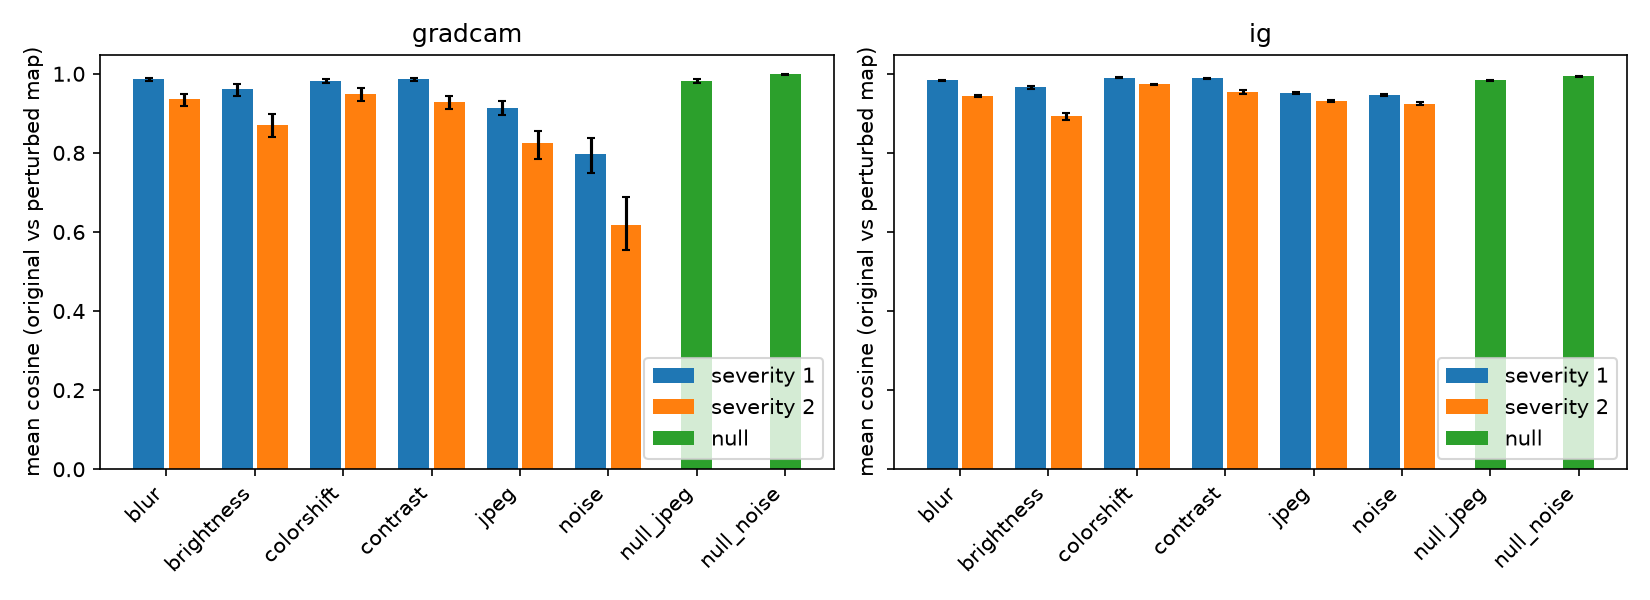
\includegraphics[width=\columnwidth]{fig_similarity.png}
\caption{Average cosine similarity of clean and perturbed attribution
maps on the validation split, by condition and severity for each method
(error bars: bootstrap 95\% CI). Null controls are green. Noise at severity
2 produces the largest collapse for Grad-CAM.}
\label{fig:sim}
\end{figure}

\textbf{The two null controls behave very differently.}
Null-noise ($\sigma{=}1$) changes just 3.6\% of predictions (2.4\% on test),
whereas \texttt{null\_jpeg} ($q{=}95$) is not inert (it changes the
predicted class in 16.3\% of validation images and 10.3\% of test images).
This unanticipated sensitivity to $q{=}95$ re-encoding was not investigated
further and may reflect low-confidence predictions near decision boundaries.
Since our excess-instability anchor averages both nulls, it is diluted; the
reported $\Delta_{\text{null}}$ understates instability relative to the
more rigorous null-noise reference. We therefore report both controls
separately rather than collapsing them.

\subsection{RQ3: Faithfulness}
Both methods beat the random control on both curves, with all 95\% CI lower
bounds above zero (Table~\ref{tab:faith}, Fig.~\ref{fig:curves}). Grad-CAM's
gaps are larger: 0.0793 [0.0435, 0.1140] on deletion and 0.1570
[0.1209, 0.1896] on insertion, compared to 0.0557 [0.0309, 0.0801] and 0.0999
[0.0716, 0.1297] for IG. H3 is supported.

The aggregate gap conceals partial coverage. Grad-CAM beats random deletion
on only 64.5\% of individual images and IG on 60.8\%; about 35--42\% of
images show no benefit over random removal (validation: Grad-CAM 35.5\%,
IG 39.2\%; test: Grad-CAM 37.6\%, IG 41.8\%). Absolute magnitudes are also
modest: the best deletion AUC is 0.348 against a random 0.428.

\begin{table}[t]
\caption{Faithfulness on the validation split ($n{=}166$). Lower deletion
AUC and higher insertion AUC indicate greater faithfulness.}
\label{tab:faith}
\centering
\footnotesize
\setlength{\tabcolsep}{3pt}
\begin{tabular}{lrr}
\toprule
Method & $\Delta_{\text{del}}$ & 95\% CI \\
\midrule
Grad-CAM & 0.079 & [0.044, 0.114] \\
IG       & 0.056 & [0.031, 0.080] \\
\midrule
Method & $\Delta_{\text{ins}}$ & 95\% CI \\
\midrule
Grad-CAM & 0.157 & [0.121, 0.190] \\
IG       & 0.100 & [0.072, 0.130] \\
\bottomrule
\end{tabular}
\end{table}

\begin{figure}[t]
\centering
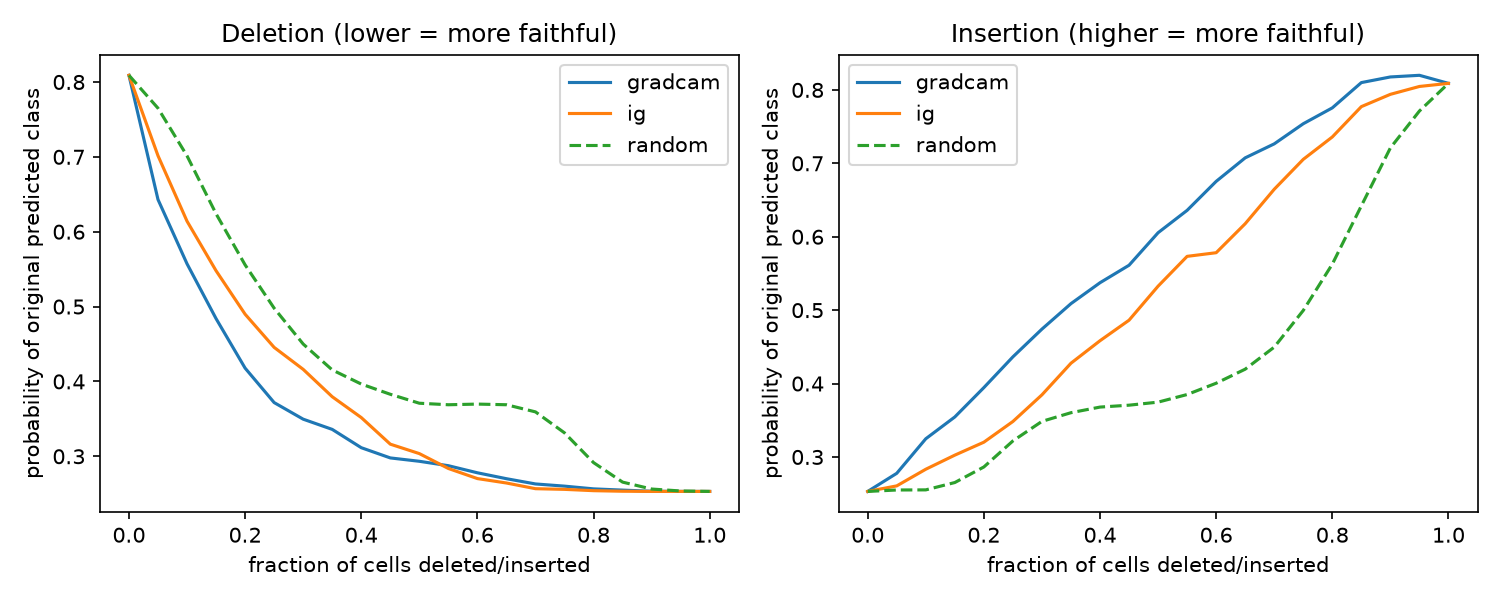
\includegraphics[width=\columnwidth]{fig_curves.png}
\caption{Validation deletion and insertion curves averaged over 166 images,
with the random-order control. Deletion: lower is better; insertion: higher
is better. Both attribution methods separate from the random control, with
modest gaps.}
\label{fig:curves}
\end{figure}

\subsection{RQ4: Error Detection via Instability}
Of the 166 validation images, 60 (36.1\%) are misclassified, providing the
positive class for the detector analysis. On the cosine instability signal,
confidence is the strongest detector at AUROC 0.7374 [0.662, 0.810],
followed by prediction flip rate at 0.6336 [0.549, 0.723], then by Grad-CAM
instability at 0.6159 [0.523, 0.690]. IG instability is 0.4731 [0.375,
0.568] (test: 0.4598 [0.359, 0.544]); since these confidence intervals
include 0.5, IG instability is indistinguishable from chance. With Spearman
the values are Grad-CAM 0.637 [0.544, 0.709] and IG 0.453 [0.353, 0.545]
(also indistinguishable from chance); the ordering relative to confidence is
unchanged. Cross-validated logistic regression gives confidence alone
0.7189, confidence plus Grad-CAM instability 0.7091 (gain $-0.0097$) and
confidence plus IG instability 0.7190 (gain $+0.00016$). H4 is not
supported: in this setting (one model, one dataset, 60 validation errors) we
found no evidence of any such added information.

The per-image correlation between $1-\cos$ and the flip rate is $+0.576$ for
Grad-CAM and $-0.287$ for IG. Grad-CAM instability carries weak marginal
error signal, but strictly less than confidence, and conditioning on
confidence removes its marginal contribution.

\subsection{Per-Class Stability}
The least rank-stable classes under Grad-CAM are \texttt{akiec} (Spearman
0.693 validation, 0.727 test) and \texttt{bcc} (0.724 validation, 0.783 test),
while melanoma (\texttt{mel}) is highly stable under Grad-CAM (Spearman
0.926 validation, the highest of any class, and 0.880 test) alongside
\texttt{nv} (0.921 validation, 0.913 test). Three caveats apply: (i) the low
Grad-CAM stability of \texttt{akiec} and \texttt{bcc} does \emph{not} hold
for IG (where \texttt{bcc} is highest at 0.876 validation / 0.855 test, and
\texttt{nv} [0.811] and \texttt{mel} [0.825] are lower); (ii) the Grad-CAM
result is partly affected by ReLU zero maps (23 validation rows in
\texttt{akiec}, 20 in \texttt{bcc}), although \texttt{akiec} and \texttt{bcc}
remain lowest under Grad-CAM after exclusion; and (iii) the rare classes
\texttt{df} ($n{=}11$) and \texttt{vasc} ($n{=}15$ validation, $14$ test) are
below $n{=}20$ and unreliable. The ordering on raw flip rate also differs
(\texttt{bkl} is highest at 44.3\%, then \texttt{akiec} 44.0\% and
\texttt{bcc} 39.0\%), since flip rate reflects the classifier's boundary
sensitivity rather than explanation stability.

\subsection{Held-Out Test Split}
Once all design decisions had been finalised, we repeated the protocol once
on the test split (165 balanced images; classification on the full 1,502
images). The main findings were directionally consistent on the held-out
test split (Table~\ref{tab:test}).

\begin{table}[t]
\caption{Validation versus held-out test. The main findings are
directionally consistent; RQ2 is a near-tie and metric-dependent on both
splits.}
\label{tab:test}
\centering
\footnotesize
\setlength{\tabcolsep}{3.5pt}
\begin{tabular}{lrr}
\toprule
Quantity & Val. & Test \\
\midrule
Accuracy & 0.793 & 0.784 \\
Balanced accuracy & 0.583 & 0.656 \\
Macro-F1 & 0.585 & 0.647 \\
Weighted-F1 & 0.796 & 0.788 \\
Flip rate (12 real) & 0.339 & 0.328 \\
Grad-CAM cos.\ / Spear. & 0.896 / 0.819 & 0.914 / 0.837 \\
IG cos.\ / Spear. & 0.954 / 0.842 & 0.951 / 0.830 \\
Confidence AUROC & 0.737 & 0.701 \\
Grad-CAM instab.\ AUROC & 0.616 & 0.629 \\
IG instab.\ AUROC & 0.473 & 0.460 \\
Grad-CAM del./ins.\ gap & 0.079 / 0.157 & 0.067 / 0.184 \\
IG del./ins.\ gap & 0.056 / 0.100 & 0.033 / 0.109 \\
\bottomrule
\end{tabular}
\end{table}

RQ1, RQ3 and RQ4 were directionally consistent on the test split. For RQ2,
under severe noise (noise, severity 2) the Grad-CAM map was all zero for
28.3\% of validation images (17.6\% on test), and only for images for which
the prediction had flipped. If these instances are scored as zero similarity,
IG appears more stable on Spearman correlation (0.736 vs.\ 0.612 on test).
If they are excluded, the two methods are statistically indistinguishable
(Grad-CAM 0.769 versus IG 0.739 on validation, and 0.743 versus 0.736 on
test, with overlapping 95\% confidence intervals), and averaged over all 12
real conditions the two are close on test even before exclusion (Grad-CAM
0.837 vs.\ IG 0.830). IG is higher on cosine similarity and Grad-CAM is
higher on top-20\% region overlap (Grad-CAM 0.675 vs.\ IG 0.548 on test).
The ranking therefore depends on the metric and on how zero maps are
handled, and we do not claim that either method is more stable. The two also
differ in map resolution and smoothing, so the comparison is not like for
like.

Test balanced accuracy exceeds validation, driven by \texttt{df} F1 0.579
vs.\ 0.270 and \texttt{vasc} 0.737 vs.\ 0.581, with \texttt{bkl} worse
(0.531 vs.\ 0.637). Given supports of 20 and 21 images for \texttt{df} and
\texttt{vasc}, this is sampling variation rather than evidence of improved
generalisation; because the checkpoint was selected on validation, the test
split gives the unbiased estimate for the metrics used for selection.

\subsection{Sensitivity Analysis: Grad-CAM Zero-Map Collapse}
When every channel-weighted activation sum is non-positive for the fixed
clean-image target class, the ReLU clamp produces an all-zero perturbed map,
which our pipeline records as $\rho{=}0$ and $\cos{=}0$ (with arbitrary tied
zero indices for top-20\% IoU). This occurs in 60/2{,}324 (2.58\%)
validation Grad-CAM rows (all within the 1{,}992 real-perturbation rows) and
37/2{,}310 (1.60\%) test rows; it is concentrated in \texttt{noise\_s2}
(47/166 validation, 28.3\%; 29/165 test, 17.6\%) and in \texttt{akiec} (23
validation, 14 test) and \texttt{bcc} (20 validation, 10 test); IG has zero
such rows.

Excluding zero-map rows (1{,}000 lesion-level bootstrap resamples, seed 0)
changes the Grad-CAM metrics as follows while leaving IG unchanged:
\begin{itemize}
\item \textbf{\texttt{noise\_s2}:} Validation Spearman rises from 0.5512
[0.4870, 0.6133] to 0.7689 [0.7153, 0.8170] ($n{=}119$), cosine from 0.6186
to 0.8629 [0.8268, 0.8968], and IoU from 0.4942 to 0.6047 [0.5620, 0.6465].
On test ($n{=}136$), Spearman rises from 0.6125 to 0.7431 [0.6918, 0.7946],
cosine from 0.6993 to 0.8484 [0.8113, 0.8846], and IoU from 0.5214 to 0.5883
[0.5471, 0.6306].
\item \textbf{\texttt{jpeg\_s2}:} Validation ($n{=}163$, 3 zero maps)
Spearman changes from 0.6826 to 0.6951 [0.6418, 0.7449], cosine from 0.8239
to 0.8391, and IoU from 0.5246 to 0.5311 (test $n{=}164$: Spearman 0.7203 to
0.7247, cosine 0.8579 to 0.8632, IoU 0.5553 to 0.5578).
\item \textbf{12-condition means:} Validation Grad-CAM Spearman rises from
0.8191 to 0.8446 [0.8245, 0.8645], cosine from 0.8960 to 0.9238 [0.9139,
0.9332], and IoU from 0.6637 to 0.6776 [0.6537, 0.7005] (test: Spearman
0.8366 to 0.8525, cosine 0.9138 to 0.9312, IoU 0.6745 to 0.6835).
\item \textbf{Per-class Grad-CAM Spearman:} On validation, \texttt{akiec}
rises from 0.6930 to 0.7440 [0.6921, 0.7892] and \texttt{bcc} from 0.7236 to
0.7694 [0.7139, 0.8193], remaining below \texttt{df} (0.8116), \texttt{bkl}
(0.8379), \texttt{vasc} (0.8897), \texttt{nv} (0.9207) and \texttt{mel}
(0.9285). On test, \texttt{akiec} rises from 0.7265 to 0.7581 and
\texttt{bcc} from 0.7832 to 0.8072 (with underpowered \texttt{df}, $n{=}11$,
at 0.7762, and \texttt{bkl}/\texttt{mel}/\texttt{nv}/\texttt{vasc} at
0.8792--0.9273).
\end{itemize}

Consequently: (a) the conclusion that IG is more stable than Grad-CAM under
\texttt{noise\_s2} on Spearman \emph{does not survive} exclusion of zero maps
(non-collapsed Grad-CAM maps reach 0.7689 validation / 0.7431 test against
IG 0.7393 / 0.7357, indicating that the steep fall in \texttt{noise\_s2}
Spearman for Grad-CAM is driven by ReLU map collapse, though IG still leads
on \texttt{noise\_s2} cosine and \texttt{jpeg\_s2} Spearman); (b)
Grad-CAM's higher top-20\% IoU \emph{survives} and strengthens; (c)
\texttt{akiec} and \texttt{bcc} being the least stable well-powered classes
under Grad-CAM \emph{survives}; and (d) the 12-condition ranking becomes
near-tied or slightly higher for Grad-CAM on Spearman (0.8446 vs.\ 0.8416
validation; 0.8525 vs.\ 0.8298 test), while IG's lead on cosine and
Grad-CAM's lead on IoU both \emph{survive}.

Across the 12 real perturbations (1,992 validation and 1,980 test
Grad-CAM rows), 100.0\% of zero-map rows have \texttt{flipped=1} (60/60
validation; 37/37 test), as opposed to 31.83\% (615/1,932) of non-zero
rows on validation and 31.55\% (613/1,943) on test. The mean
post-perturbation probability assigned to the original clean-image predicted
class (\texttt{conf\_orig\_class\_after}) is 0.000524 (0.052\%) for zero-map
rows versus 0.636448 (63.64\%) for non-zero rows on validation, and 0.000288
(0.029\%) for zero-map rows compared to 0.644600 (64.46\%) for non-zero rows on
test. Within non-zero-map Grad-CAM rows at \texttt{noise\_s2}, rows with
\texttt{flipped=0} have mean Spearman 0.8480 ($n{=}61$) on validation
and 0.8640 ($n{=}58$) on test, while those with \texttt{flipped=1} have
mean Spearman 0.6857 ($n{=}58$) on validation and 0.6532 ($n{=}78$) on test.
Zero-map collapse therefore coincided with a prediction flip in every instance
(60/60 on validation, 37/37 on test), with near-zero probability for the
original class, so it reflects the model withdrawing its evidence for that
class rather than a numerical failure at random. Because the protocol explains
the original class, Grad-CAM (which keeps only positive evidence through a
ReLU) can collapse to an all-zero map while IG cannot; this is a
protocol-dependent difference between the methods. Excluding zero maps
conditions the comparison on cases where the model retained some evidence
for the original class, which favours Grad-CAM, so we report both versions.
Among non-zero maps, rank correlation was lower when the prediction flipped
(0.69 validation, 0.65 test) than when it did not (0.85, 0.86), so
explanation change largely tracks prediction change.

\section{Discussion}

The strongest finding is methodological rather than clinical: the verdict on
which explanation method is ``more stable'' depends on the metric. Global
rank correlation and local top-region overlap disagree systematically, and
the two methods' maps differ in resolution and smoothing (Grad-CAM $7\times7$
upsampled vs.\ IG pixel-level Gaussian-smoothed), so cross-method comparisons
are not like for like. Any single-number stability claim is therefore
incomplete, and reporting all three metrics should be the default.

Second, in this setting (one model, one dataset, 60 validation errors and 51
test errors) we found no evidence that explanation instability adds
information beyond model confidence for error detection, and IG instability
AUROC is indistinguishable from chance. Softmax confidence is therefore an
important baseline to beat when evaluating perturbation-based explanation
signals.

Third, the \texttt{null\_jpeg} ($q{=}95$) control was not inert: it changed
the predicted class in 16.3\% of validation images (10.3\% on test). We did
not investigate this further, and it may reflect low-confidence predictions
near the decision boundary, showing that controls assumed to be harmless
should be empirically verified.

Finally, we found no detectable association between per-image stability and
faithfulness (Spearman about 0.04, $n{=}166$), supporting the practice of
measuring stability and faithfulness as separate properties.

\section{Limitations}
\begin{enumerate}
\item \emph{Single model and single dataset.} Results are specific to one
architecture (ResNet-18) and one dataset (HAM10000); other architectures or
clinical cohorts may differ.
\item \emph{Small error sample size for RQ4.} The XAI samples contain only 60
(validation) and 51 (test) misclassified images, with 3 to 14 errors per
class, which limits statistical power for error-detection AUROC comparisons.
\item \emph{Underpowered rare classes.} In the XAI sample, \texttt{df}
($n{=}11$) and \texttt{vasc} ($n{=}15$ validation, $14$ test) are below $n{=}20$
and their per-class estimates are unreliable.
\item \emph{Class-balanced XAI sampling vs.\ population error rate.} Because
the XAI sample is class-balanced (up to 28 images per class), the sample
error rate (36.1\% validation, 30.9\% test) is not the population error rate
on the full splits (20.7\% validation, 21.6\% test).
\item \emph{Cross-method resolution and smoothing difference.} Grad-CAM uses
a $7\times7$ activation map bilinearly upsampled to $224\times224$, whereas
IG is computed at pixel resolution and Gaussian-smoothed ($11\times11$,
$\sigma{=}3$), so cross-method comparisons are not strictly like for like.
\item \emph{Grad-CAM ReLU zero-map collapse.} All-zero perturbed Grad-CAM
maps after ReLU occur in 60/2,324 validation and 37/2,310 test rows
(concentrated in \texttt{noise\_s2} and in \texttt{akiec} and \texttt{bcc}),
recorded as $\rho{=}0$ and $\cos{=}0$ via zero-map collapse (Sec.~IV-H).
\item \emph{No multiple-comparison correction.} Many 95\% bootstrap
confidence intervals are reported across conditions, metrics, methods and
classes without multiple-testing adjustment.
\item \emph{Imperfect nulls.} The \texttt{null\_jpeg} ($q{=}95$) control is
not inert (changing 16.3\% validation / 10.3\% test predictions), diluting the
two-null average anchor.
\item \emph{Coarse faithfulness grid, synthetic perturbations, single seed,
and no clinician ground truth.} Deletion and insertion operate on a
$28\times28$ grid of $8\times8$-pixel cells without retraining (ROAR
\cite{hooker2019}) or clinician-annotated lesion masks; perturbations are
synthetic, and only one training seed was evaluated.
\item \emph{IG input-structure inheritance and no parameter-randomisation check.}
IG with a zero baseline multiplies attributions by the input, so its maps can
inherit image structure independently of the model; prior sanity-check
studies report that global IG on images is only weakly sensitive to model
parameters. Its apparent stability under perturbations may therefore partly
reflect the input itself, and we did not run parameter-randomisation checks
on our own model.
\end{enumerate}

\section{Conclusion}
We measured, on a leak-free HAM10000 split, both the stability and the
faithfulness of Grad-CAM and Integrated Gradients explanations for a
ResNet-18 lesion classifier, calibrating instability against null controls
and testing its value as an error detector:
\begin{itemize}
\item Noise is the most disruptive perturbation for predictions (it flips
about 63\% of validation predictions at severity 2). For explanations, noise
is the most disruptive condition when all-zero Grad-CAM maps are scored as zero
similarity. The \texttt{null\_jpeg} ($q{=}95$) control is not inert (it changes
16.3\% of validation predictions; 10.3\% on test; not investigated
further, possibly reflecting low-confidence predictions near decision
boundaries).
\item H2 was partly supported. Both methods changed far more under
severity-2 perturbations than under the null controls, but IG was not less
stable than Grad-CAM. Under severe noise, the Grad-CAM map was all zero
for 28.3\% of validation images (17.6\% on test), and only for images whose
prediction had flipped. If these cases are scored as zero similarity, IG
appears more stable on Spearman correlation. If they are excluded, the two
methods are statistically indistinguishable (Grad-CAM 0.769 versus IG 0.739
on validation, with overlapping 95\% confidence intervals). IG is higher on
cosine similarity and Grad-CAM is higher on top-20\% region overlap, so we
do not claim that either method is more stable. The two also differ
in map resolution and smoothing, so they are not directly comparable.
\item Both methods beat random deletion and insertion with 95\% confidence
intervals excluding zero, though the absolute gaps are small and about
35 to 42\% of images show no benefit over random removal. We found no
detectable association between per-image stability and faithfulness
(Spearman about 0.04, $n{=}166$).
\item In this setting (one model, one dataset, 60 validation errors and 51
test errors) we found no evidence that explanation instability adds
information beyond model confidence for error detection, and IG instability
AUROC is indistinguishable from chance.
\item Under Grad-CAM, \texttt{akiec} and \texttt{bcc} have the lowest
explanation stability (partly through zero maps, though the ordering
survives exclusion), while melanoma (\texttt{mel}) is highly stable under
Grad-CAM; the low stability of \texttt{akiec} and \texttt{bcc} does not
hold for IG, and the rare classes \texttt{df} ($n{=}11$) and \texttt{vasc} (14--15)
are below $n{=}20$ and unreliable.
\item The main findings were directionally consistent on the held-out test
split. The RQ2 comparison between the two methods was a near-tie and
metric-dependent, and the per-class ordering under IG differed from Grad-CAM.
\end{itemize}

Future work should run multiple training seeds to separate perturbation
instability from training variance, replace the improvised nulls with a
verified null battery, test grid-granularity sensitivity, and add
clinician-annotated lesion masks to convert internal faithfulness into
clinical plausibility.

\section*{Acknowledgements}
The authors thank the creators of the HAM10000 dataset for making the
dermoscopic imagery and clinical metadata publicly available for academic
research. Our experimental pipeline was built using open-source Python
libraries, including PyTorch, Torchvision, NumPy, SciPy, scikit-learn, and
Matplotlib. Generative AI tools were used in a limited capacity for
code debugging and language polishing during manuscript preparation;
the authors designed the experiments, verified all empirical results, and
take full responsibility for the content of this report.

\begin{thebibliography}{10}

\bibitem{esteva2017}
A.~Esteva \emph{et al.}, ``Dermatologist-level classification of skin cancer
with deep neural networks,'' \emph{Nature}, vol.~542, no.~7639,
pp.~115--118, 2017.

\bibitem{selvaraju2017}
R.~R. Selvaraju, M.~Cogswell, A.~Das, R.~Vedantam, D.~Parikh, and
D.~Batra, ``Grad-CAM: Visual explanations from deep networks via
gradient-based localization,'' in \emph{Proc. IEEE Int. Conf. Comput. Vis.
(ICCV)}, 2017, pp.~618--626.

\bibitem{sundararajan2017}
M.~Sundararajan, A.~Taly, and Q.~Yan, ``Axiomatic attribution for deep
networks,'' in \emph{Proc. Int. Conf. Mach. Learn. (ICML)}, 2017,
pp.~3319--3328.

\bibitem{adebayo2018}
J.~Adebayo, J.~Gilmer, M.~Muelly, I.~Goodfellow, M.~Hardt, and B.~Kim,
``Sanity checks for saliency maps,'' in \emph{Adv. Neural Inf. Process.
Syst. (NeurIPS)}, 2018.

\bibitem{ghorbani2019}
A.~Ghorbani, A.~Abid, and J.~Zou, ``Interpretation of neural networks is
fragile,'' in \emph{Proc. AAAI Conf. Artif. Intell. (AAAI)}, 2019.

\bibitem{saarela2022}
M.~Saarela and L.~Georgieva, ``Robustness, stability, and fidelity of
explanations for a deep skin cancer classification model,''
\emph{Applied Sciences}, vol.~12, no.~19, art.~9545, 2022.

\bibitem{arun2021}
N.~Arun \emph{et al.}, ``Assessing the trustworthiness of saliency maps
for localizing abnormalities in medical imaging,''
\emph{Radiology: Artificial Intelligence}, vol.~3, no.~6, art.~e200267, 2021.

\bibitem{paxton2025}
K.~Paxton, K.~Aslansefat, A.~Akagi\'c, D.~Thakker, and
Y.~Papadopoulos, ``Safer skin lesion classification with global class
activation probability map evaluation and SafeML,'' arXiv:2508.20776, 2025.

\bibitem{zhang2024}
J.~Zhang, H.~Chao, G.~Dasegowda, G.~Wang, M.~K. Kalra, and
P.~Yan, ``Revisiting the trustworthiness of saliency methods in
radiology AI,'' \emph{Radiology: Artificial Intelligence}, vol.~6, no.~1,
art.~e220221, 2024, doi:10.1148/ryai.220221.

\bibitem{hooker2019}
S.~Hooker, D.~Erhan, P.-J. Kindermans, and B.~Kim, ``A benchmark for
interpretability methods in deep neural networks,'' in \emph{Adv. Neural
Inf. Process. Syst. (NeurIPS)}, 2019.

\bibitem{petsiuk2018}
V.~Petsiuk, A.~Das, and K.~Saenko, ``RISE: Randomized input sampling for
explanation of black-box models,'' in \emph{Proc. British Mach. Vis. Conf.
(BMVC)}, 2018.

\bibitem{tschandl2018}
P.~Tschandl, C.~Rosendahl, and H.~Kittler, ``The HAM10000 dataset, a large
collection of multi-source dermatoscopic images of common pigmented skin
lesions,'' \emph{Scientific Data}, vol.~5, art.~180161, 2018.

\bibitem{he2016}
K.~He, X.~Zhang, S.~Ren, and J.~Sun, ``Deep residual learning for image
recognition,'' in \emph{Proc. IEEE Conf. Comput. Vis. Pattern Recognit.
(CVPR)}, 2016, pp.~770--778.

\bibitem{loshchilov2019}
I.~Loshchilov and F.~Hutter, ``Decoupled weight decay regularization,'' in
\emph{Proc. Int. Conf. Learn. Represent. (ICLR)}, 2019.

\end{thebibliography}

\end{document}
